\chapter{Protocole expérimental et benchmarking}

\epigraph{\textit{``In God we trust, all others must bring data.''}}{--- W. Edwards Deming}

\section{Environnement d'exécution}

\subsection{Supercalculateur Romeo}

Les expérimentations ont été réalisées sur le supercalculateur \textbf{Romeo} de l'Université de Reims Champagne-Ardenne, membre du mésocentre de calcul régional. Romeo est un cluster hétérogène de nouvelle génération combinant des architectures x86 et ARM.

\begin{table}[H]
\centering
\begin{tabular}{ll}
\toprule
\textbf{Caractéristique} & \textbf{Valeur} \\
\midrule
Cluster & Romeo (URCA) \\
Gestionnaire de ressources & SLURM \\
Réseau d'interconnexion & InfiniBand HDR \\
Système de fichiers & Lustre (scratch partagé) \\
Nombre total de nœuds & 102 (58 ARM + 44 x86) \\
Cœurs CPU totaux & $\sim$25\,000 \\
\bottomrule
\end{tabular}
\caption{Caractéristiques générales du supercalculateur Romeo}
\label{tab:romeo_general}
\end{table}

\subsection{Partitions et politiques d'ordonnancement}

Romeo propose trois partitions avec des limites de temps différentes :

\begin{table}[H]
\centering
\begin{tabular}{lcccp{4cm}}
\toprule
\textbf{Partition} & \textbf{Nœuds ARM} & \textbf{Nœuds x86} & \textbf{Total} & \textbf{Usage} \\
\midrule
\texttt{instant} (défaut) & 58 & 44 & 102 & Jobs courts, tests interactifs \\
\texttt{short} & 56 & 43 & 99 & Jobs de quelques heures \\
\texttt{long} & 40 & 24 & 64 & Jobs longs (jours) \\
\bottomrule
\end{tabular}
\caption{Partitions disponibles sur Romeo}
\label{tab:romeo_partitions}
\end{table}

\subsection{Quotas et limites de ressources}

L'accès aux ressources de calcul est contrôlé par un système de quotas associé à chaque compte utilisateur. Ces quotas limitent le nombre total de CPUs utilisables simultanément :

\begin{table}[H]
\centering
\begin{tabular}{lc}
\toprule
\textbf{Paramètre} & \textbf{Valeur} \\
\midrule
Limite CPUs simultanés (GrpCPUs) & 400 \\
Nœuds x86 max (192 CPUs/nœud) & 2 \\
Nœuds ARM max (288 CPUs/nœud) & 1 \\
\bottomrule
\end{tabular}
\caption{Quotas de ressources pour le compte projet}
\label{tab:quotas}
\end{table}

Cette limite de 400 CPUs simultanés impose des contraintes sur l'exécution parallèle des benchmarks : un job ARM utilisant 192 CPUs empêche le lancement simultané d'un job MPI multi-nœuds (2 nœuds $\times$ 192 CPUs = 384 CPUs supplémentaires dépasserait le quota). Les jobs sont alors placés en file d'attente avec le statut \texttt{AssocGrpCpuLimit} jusqu'à libération des ressources.

\subsection{Architecture des nœuds de calcul}

Romeo dispose de deux familles de nœuds aux caractéristiques distinctes :

\subsubsection{Nœuds ARM : NVIDIA Grace (romeo-a*)}

Les nœuds ARM sont équipés de processeurs \textbf{NVIDIA Grace} basés sur l'architecture \textbf{ARM Neoverse-V2}. Chaque nœud intègre également 4 GPUs NVIDIA H100 pour l'accélération GPU.

\begin{table}[H]
\centering
\begin{tabular}{ll}
\toprule
\textbf{Caractéristique} & \textbf{Valeur} \\
\midrule
Processeur & NVIDIA Grace (ARM Neoverse-V2) \\
Nœuds disponibles & 58 (romeo-a001 à romeo-a058) \\
Sockets & 4 \\
Cœurs par socket & 72 \\
Cœurs totaux par nœud & 288 (4 × 72 × 1) \\
Threads par cœur & 1 (pas d'hyperthreading) \\
Mémoire RAM & 800 Go (LPDDR5X) \\
GPUs & 4 × NVIDIA H100 \\
\bottomrule
\end{tabular}
\caption{Spécifications des nœuds ARM (romeo-a*)}
\label{tab:romeo_arm}
\end{table}

\subsubsection{Nœuds x86 : AMD EPYC 9654 (romeo-c*)}

Les nœuds x86 utilisent des processeurs \textbf{AMD EPYC 9654} (architecture Zen 4, Genoa). Ces nœuds sont optimisés pour le calcul CPU intensif sans accélération GPU.

\begin{table}[H]
\centering
\begin{tabular}{ll}
\toprule
\textbf{Caractéristique} & \textbf{Valeur} \\
\midrule
Processeur & AMD EPYC 9654 (Zen 4, Genoa) \\
Nœuds disponibles & 44 (romeo-c001 à romeo-c040, romeo-c101 à romeo-c104) \\
Sockets & 2 \\
Cœurs par socket & 96 \\
Cœurs totaux par nœud & 192 (2 × 96 × 1) \\
Threads par cœur & 1 (SMT désactivé) \\
Mémoire RAM & 1,1 To (DDR5-4800) \\
Cache L3 & 384 Mo (2 × 192 Mo) \\
Fréquence & 2,4 GHz (base) / 3,7 GHz (boost) \\
Domaines NUMA & 2 (1 par socket) \\
\bottomrule
\end{tabular}
\caption{Spécifications des nœuds x86 (romeo-c*)}
\label{tab:romeo_x86}
\end{table}

\subsubsection{Comparaison des architectures}

\begin{table}[H]
\centering
\begin{tabular}{lcc}
\toprule
\textbf{Caractéristique} & \textbf{ARM (Grace)} & \textbf{x86 (EPYC 9654)} \\
\midrule
Architecture ISA & ARMv9 (Neoverse-V2) & x86-64 (Zen 4) \\
Cœurs/nœud & 288 & 192 \\
Sockets & 4 & 2 \\
Décodage instructions & 10-wide & 6-wide \\
Mémoire type & LPDDR5X & DDR5-4800 \\
Latence L1 & 3 cycles & 4 cycles \\
Pipeline & Out-of-order, 10 étages & Out-of-order, 19 étages \\
GPUs intégrés & 4 × H100 & Aucun \\
\bottomrule
\end{tabular}
\caption{Comparaison des architectures ARM et x86}
\label{tab:arch_comparison}
\end{table}

\begin{figure}[H]
\centering
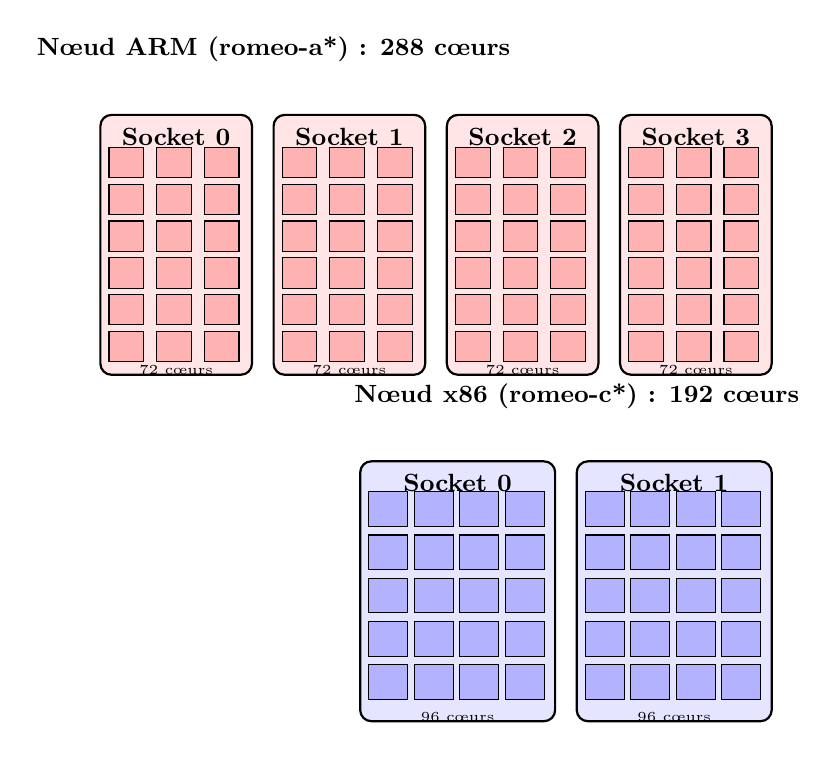
\begin{tikzpicture}[scale=0.55, every node/.style={font=\small}]
    % ARM Node
    \node[anchor=south] at (4, 7) {\textbf{Nœud ARM (romeo-a*) : 288 cœurs}};
    \foreach \s in {0,1,2,3} {
        \draw[thick, rounded corners, fill=red!10] (\s*4, 0) rectangle (\s*4+3.5, 6);
        \node at (\s*4+1.75, 5.5) {\textbf{Socket \s}};
        \foreach \y in {0,...,5} {
            \foreach \x in {0,...,2} {
                \draw[fill=red!30] (\s*4+0.2+\x*1.1, 0.3+\y*0.85) rectangle (\s*4+1+\x*1.1, 1+\y*0.85);
            }
        }
        \node[font=\tiny] at (\s*4+1.75, 0.1) {72 cœurs};
    }

    % x86 Node
    \node[anchor=south] at (11, -1) {\textbf{Nœud x86 (romeo-c*) : 192 cœurs}};
    \foreach \s in {0,1} {
        \draw[thick, rounded corners, fill=blue!10] (6+\s*5, -8) rectangle (6+\s*5+4.5, -2);
        \node at (6+\s*5+2.25, -2.5) {\textbf{Socket \s}};
        \foreach \y in {0,...,4} {
            \foreach \x in {0,...,3} {
                \draw[fill=blue!30] (6+\s*5+0.2+\x*1.05, -7.5+\y*1) rectangle (6+\s*5+1.1+\x*1.05, -6.7+\y*1);
            }
        }
        \node[font=\tiny] at (6+\s*5+2.25, -7.9) {96 cœurs};
    }
\end{tikzpicture}
\caption{Topologie des nœuds ARM (4 sockets × 72 cœurs) et x86 (2 sockets × 96 cœurs)}
\label{fig:node_topology}
\end{figure}

\subsection{Compilation}

Tous les binaires sont compilés avec des optimisations agressives adaptées à l'architecture cible :

\begin{lstlisting}[language=bash, caption={Flags de compilation}]
# Compilateur
CXX = g++ (GCC 12+)
MPICXX = mpicxx (OpenMPI)

# Flags d'optimisation
OPTFLAGS = -O3 -march=native -mtune=native \
           -funroll-loops -fomit-frame-pointer -flto

# Standard et flags supplementaires
CXXFLAGS = -std=c++20 $(OPTFLAGS) -fopenmp \
           -Wall -Wextra -DNDEBUG
\end{lstlisting}

\begin{table}[H]
\centering
\begin{tabular}{lp{8cm}}
\toprule
\textbf{Flag} & \textbf{Effet} \\
\midrule
\texttt{-O3} & Optimisations agressives (inlining, vectorisation) \\
\texttt{-march=native} & Instructions spécifiques au CPU hôte (AVX-512, etc.) \\
\texttt{-mtune=native} & Scheduling optimisé pour le CPU hôte \\
\texttt{-funroll-loops} & Déroulage automatique des boucles \\
\texttt{-flto} & Link-Time Optimization (optimisation globale) \\
\texttt{-DNDEBUG} & Désactive les assertions \\
\bottomrule
\end{tabular}
\caption{Flags de compilation et leurs effets}
\label{tab:compilation_flags}
\end{table}

\subsection{Affinité des threads}

L'affinité des threads est contrôlée via les variables OpenMP et les options SLURM :

\begin{lstlisting}[language=bash, caption={Configuration de l'affinité}]
# Variables OpenMP
export OMP_PLACES=cores      # Un thread par coeur physique
export OMP_PROC_BIND=close   # Threads proches (meme socket)
export OMP_STACKSIZE=16M     # Pile pour la recursion profonde

# Options SLURM
srun --cpu-bind=cores \
     --distribution=block:block \
     ./binary
\end{lstlisting}

\begin{figure}[H]
\centering
\begin{tikzpicture}[scale=0.7]
    % Socket 0
    \draw[thick, rounded corners, fill=burgundy!10] (0,0) rectangle (7,3);
    \node at (3.5, 2.5) {\textbf{Socket 0 (NUMA 0)}};
    \foreach \x in {0,...,5} {
        \draw[fill=gold!50] (0.5+\x*1.1, 0.5) rectangle (1.3+\x*1.1, 1.8);
        \node[font=\tiny] at (0.9+\x*1.1, 1.15) {C\x};
    }
    \node at (3.5, 0.2) {\tiny ... 96 cœurs};

    % Socket 1
    \draw[thick, rounded corners, fill=blue!10] (8,0) rectangle (15,3);
    \node at (11.5, 2.5) {\textbf{Socket 1 (NUMA 1)}};
    \foreach \x in {0,...,5} {
        \draw[fill=blue!30] (8.5+\x*1.1, 0.5) rectangle (9.3+\x*1.1, 1.8);
        \node[font=\tiny] at (8.9+\x*1.1, 1.15) {C\x};
    }
    \node at (11.5, 0.2) {\tiny ... 96 cœurs};

    % Légende binding
    \node at (7.5, -1) {\textbf{close} : threads regroupés sur un socket};
    \node at (7.5, -1.8) {\textbf{spread} : threads répartis sur les deux sockets};
\end{tikzpicture}
\caption{Topologie NUMA et stratégies de binding}
\label{fig:numa_topology}
\end{figure}

\section{Paramétrage des expériences}

\subsection{Valeurs de $n$ testées}

Les expériences couvrent plusieurs ordres de grandeur de difficulté :

\begin{table}[H]
\centering
\begin{tabular}{cccp{5cm}}
\toprule
\textbf{$n$} & \textbf{$L^*(n)$} & \textbf{Temps typ. (1 thread)} & \textbf{Usage} \\
\midrule
9 & 44 & $\sim$15 ms & Validation, warm-up \\
10 & 55 & $\sim$120 ms & Tests rapides \\
11 & 72 & $\sim$2.5 s & Scalabilité faible \\
12 & 85 & $\sim$20 s & Benchmark principal \\
13 & 106 & $\sim$6-7 min & Benchmark principal \\
14 & 127 & $\sim$heures & Stress test \\
\bottomrule
\end{tabular}
\caption{Ordres testés et temps d'exécution typiques (V1 séquentiel)}
\label{tab:tested_n}
\end{table}

\subsection{Initialisation de la borne}

La borne supérieure initiale $bestLen$ est cruciale pour l'efficacité de l'élagage :

\begin{lstlisting}[language=C++, caption={Initialisation de bestLen}]
// Longueurs optimales connues (lookup table)
int knownOptimal[] = {0, 0, 1, 3, 6, 11, 17, 25, 34, 44,
                      55, 72, 85, 106, 127};

// Initialisation
int maxLen = (n <= 14) ? knownOptimal[n] : (n * n);
\end{lstlisting}

\begin{important}{Impact de l'initialisation}
Initialiser avec la longueur optimale connue ($L^*(n)$) ne \textit{triche} pas : l'algorithme doit quand même prouver qu'aucune solution plus courte n'existe. Cela évite simplement d'explorer des branches menant à des solutions sous-optimales.
\end{important}

\subsection{Configurations de threads (OpenMP)}

\begin{table}[H]
\centering
\begin{tabular}{cl}
\toprule
\textbf{Threads} & \textbf{Justification} \\
\midrule
8 & Baseline, un seul domaine NUMA partiel \\
16 & Scaling intra-NUMA \\
32 & Scaling intra-NUMA \\
64 & Proche saturation d'un socket \\
96 & Un socket complet \\
192 & Deux sockets complets \\
\bottomrule
\end{tabular}
\caption{Configurations de threads testées}
\label{tab:thread_configs}
\end{table}

\subsection{Configurations MPI hybrides}

Pour les benchmarks MPI+OpenMP, nous avons sélectionné des configurations optimales plutôt que de tester toutes les combinaisons possibles. L'objectif est de maximiser l'utilisation des ressources tout en minimisant l'overhead de communication.

\paragraph{Critères de sélection.}
\begin{itemize}
    \item \textbf{Total workers constant} : chaque configuration utilise le même nombre total de workers ($\text{MPI} \times \text{threads} = 192$ pour 2 nœuds)
    \item \textbf{Puissances de 2} : le nombre de processus MPI est une puissance de 2 pour supporter l'algorithme hypercube (V1, V2)
    \item \textbf{Granularité variable} : de gros grains (peu de MPI, beaucoup de threads) à fins grains (beaucoup de MPI, peu de threads)
\end{itemize}

\begin{table}[H]
\centering
\begin{tabular}{cccp{5cm}}
\toprule
\textbf{MPI} & \textbf{Threads} & \textbf{Total} & \textbf{Configuration} \\
\midrule
1 & 96 & 96 & Baseline single-node (OpenMP pur) \\
2 & 96 & 192 & 1 proc/nœud (optimal NUMA) \\
4 & 48 & 192 & 2 proc/nœud \\
8 & 24 & 192 & 4 proc/nœud \\
16 & 12 & 192 & 8 proc/nœud (x86 seulement) \\
\bottomrule
\end{tabular}
\caption{Configurations MPI hybrides optimales testées}
\label{tab:mpi_configs}
\end{table}

\paragraph{Justification.}
La configuration 2 MPI $\times$ 96 threads (1 processus par nœud) est théoriquement optimale car elle minimise les communications inter-nœuds tout en maximisant le parallélisme OpenMP intra-nœud. Les configurations avec plus de processus MPI permettent d'évaluer l'overhead de communication et l'impact de la granularité sur les performances.

\section{Métriques de performance}

\subsection{Temps d'exécution}

Le temps d'exécution est mesuré avec la bibliothèque \texttt{<chrono>} de C++ :

\begin{lstlisting}[language=C++, caption={Mesure du temps d'exécution}]
#include <chrono>

auto start = std::chrono::high_resolution_clock::now();

// Appel a l'algorithme
searchGolombV5(n, maxLen, best, prefixDepth);

auto end = std::chrono::high_resolution_clock::now();
double elapsed = std::chrono::duration<double>(end - start).count();
\end{lstlisting}

Le temps mesuré inclut :
\begin{itemize}
    \item Génération des préfixes (si applicable)
    \item Exploration parallèle
    \item Synchronisations MPI (si applicable)
    \item Fusion des résultats
\end{itemize}

\subsection{Speedup}

Le \textbf{speedup} mesure l'accélération obtenue par la parallélisation :

\begin{equation}
S(p) = \frac{T_1}{T_p}
\end{equation}

où $T_1$ est le temps avec 1 thread/processus et $T_p$ le temps avec $p$ threads/processus.

\begin{itemize}
    \item \textbf{Speedup idéal} : $S(p) = p$ (scaling linéaire)
    \item \textbf{Speedup super-linéaire} : $S(p) > p$ (effets de cache)
    \item \textbf{Speedup sous-linéaire} : $S(p) < p$ (surcoûts, contention)
\end{itemize}

\subsection{Efficacité parallèle}

L'\textbf{efficacité} normalise le speedup par le nombre de processeurs :

\begin{equation}
E(p) = \frac{S(p)}{p} = \frac{T_1}{p \cdot T_p}
\end{equation}

\begin{itemize}
    \item $E(p) = 100\%$ : efficacité parfaite
    \item $E(p) > 60\%$ : généralement considéré acceptable
    \item $E(p) < 50\%$ : surcoûts significatifs
\end{itemize}

\subsection{États explorés}

Le nombre d'\textbf{états explorés} compte les nœuds de l'arbre de recherche visités :

\begin{lstlisting}[language=C++, caption={Comptage des états explorés}]
static std::atomic<long long> exploredCount{0};

void backtrackIterative(...) {
    while (stackTop >= 0) {
        localExplored++;  // Compteur local (evite contention)
        // ...
    }
}

// Agregation finale
exploredCount.fetch_add(localExplored, std::memory_order_relaxed);
\end{lstlisting}

Cette métrique permet de calculer :
\begin{itemize}
    \item \textbf{Débit} : $\text{États/sec} = \frac{\text{États explorés}}{\text{Temps}}$
    \item \textbf{Efficacité algorithmique} : moins d'états explorés = meilleur élagage
\end{itemize}

\subsection{Résumé des métriques}

\begin{table}[H]
\centering
\begin{tabular}{llp{5cm}}
\toprule
\textbf{Métrique} & \textbf{Formule} & \textbf{Interprétation} \\
\midrule
Temps (s) & $T_p$ & Durée totale d'exécution \\
Speedup & $S(p) = T_1 / T_p$ & Accélération vs séquentiel \\
Efficacité (\%) & $E(p) = 100 \cdot S(p) / p$ & Utilisation des ressources \\
États explorés & $N$ & Travail effectué \\
Débit (états/s) & $N / T_p$ & Vitesse de traitement \\
\bottomrule
\end{tabular}
\caption{Récapitulatif des métriques de performance}
\label{tab:metrics_summary}
\end{table}

\section{Traitement des résultats}

\subsection{Format des fichiers CSV}

Les résultats sont exportés au format CSV pour faciliter l'analyse. Deux formats sont utilisés :

\subsubsection{Format OpenMP}

\begin{lstlisting}[basicstyle=\tiny\ttfamily, caption={En-tête CSV OpenMP}]
threads,n,version,binding,time_s,length,states,states_per_sec
8,12,V5,close,2.543,85,264788630,1.04e+08
16,12,V5,close,1.287,85,264788630,2.06e+08
...
\end{lstlisting}

\subsubsection{Format MPI}

\begin{lstlisting}[basicstyle=\tiny\ttfamily, caption={En-tête CSV MPI}]
mpi_procs,threads,total_workers,n,version,time_s,length,states,states_per_sec
4,24,96,13,V3,12.456,106,4251895005,3.41e+08
...
\end{lstlisting}

\subsection{Parsing et extraction}

Les scripts SLURM incluent des fonctions de parsing robustes :

\begin{lstlisting}[language=bash, caption={Extraction des métriques depuis la sortie}]
# Fonction de parsing
parse_output() {
    local output="$1"
    local field="$2"
    echo "$output" | grep -E "^${field}\s*:" | \
         sed -E "s#^${field}\s*:\s*##" | awk '{print $1}'
}

# Usage
output=$(run_bench "$binary" "$n" "$threads")
time_val=$(parse_output "$output" "Time")
len_val=$(parse_output "$output" "Length")
states_val=$(parse_output "$output" "States")
\end{lstlisting}

\subsection{Génération des graphiques}

Les données CSV peuvent être visualisées avec Python/Matplotlib ou tout outil d'analyse :

\begin{lstlisting}[language=Python, caption={Exemple de script de visualisation}]
import pandas as pd
import matplotlib.pyplot as plt

# Charger les donnees
df = pd.read_csv('results_v1v2v3v4v5_comparison.csv')

# Filtrer pour V5 et binding=close
df_v5 = df[(df['version'] == 'V5') & (df['binding'] == 'close')]

# Graphique speedup
for n in [12, 13]:
    subset = df_v5[df_v5['n'] == n]
    baseline = subset[subset['threads'] == 8]['time_s'].values[0]
    speedup = baseline / subset['time_s']
    plt.plot(subset['threads'], speedup, label=f'n={n}')

plt.xlabel('Threads')
plt.ylabel('Speedup')
plt.legend()
plt.savefig('speedup_openmp.pdf')
\end{lstlisting}

\begin{figure}[H]
\centering
\begin{tikzpicture}[scale=0.8]
    \begin{axis}[
        xlabel={Nombre de threads},
        ylabel={Speedup},
        grid=major,
        width=10cm,
        height=6cm,
        legend pos=north west,
        xmin=0, xmax=200,
        ymin=0,
    ]
    % Ideal
    \addplot[thick, dashed, gray, domain=8:192] {x/8};
    \addlegendentry{Idéal}

    % Courbe conceptuelle n=12
    \addplot[thick, burgundy, mark=*] coordinates {
        (8, 1) (16, 1.9) (32, 3.6) (64, 6.5) (96, 8.5) (192, 12)
    };
    \addlegendentry{$n=12$}

    % Courbe conceptuelle n=13
    \addplot[thick, gold, mark=square*] coordinates {
        (8, 1) (16, 1.95) (32, 3.8) (64, 7.2) (96, 10) (192, 16)
    };
    \addlegendentry{$n=13$}
    \end{axis}
\end{tikzpicture}
\caption{Exemple de graphique de speedup (valeurs illustratives)}
\label{fig:speedup_example}
\end{figure}

\subsection{Analyses automatisées}

Les scripts SLURM génèrent automatiquement plusieurs analyses :

\begin{enumerate}
    \item \textbf{Comparaison des versions} : V1 vs V2 vs V3 vs V4 vs V5
    \item \textbf{Impact du binding} : close vs spread
    \item \textbf{Scaling NUMA} : comportement au-delà d'un socket
    \item \textbf{Scaling MPI} : hypercube vs Allreduce
\end{enumerate}

\begin{lstlisting}[language=bash, caption={Génération automatique des résumés}]
# Exemple de sortie automatique
echo "=========================================="
echo "SUMMARY - V5 vs others (close binding)"
echo "=========================================="

printf "%-8s %-4s %-10s %-10s %-10s\n" \
    "Threads" "n" "V1(s)" "V5(s)" "Speedup"

for t in 8 16 32 64 96 192; do
    for n in 12 13; do
        v1_time=$(grep "^$t,$n,V1,close," "$CSV_FILE" | cut -d',' -f5)
        v5_time=$(grep "^$t,$n,V5,close," "$CSV_FILE" | cut -d',' -f5)
        speedup=$(echo "scale=2; $v1_time / $v5_time" | bc)
        printf "%-8s %-4s %-10s %-10s %-10s\n" \
            "$t" "$n" "$v1_time" "$v5_time" "${speedup}x"
    done
done
\end{lstlisting}

\subsection{Reproductibilité}

Pour assurer la reproductibilité des résultats :

\begin{enumerate}
    \item \textbf{Mode exclusif} : \texttt{--exclusive} réserve le nœud complet
    \item \textbf{Scratch local} : travail dans \texttt{/scratch\_p/\$USER/\$SLURM\_JOBID}
    \item \textbf{Recompilation} : binaires reconstruits à chaque job
    \item \textbf{Timestamping} : date/heure enregistrées dans les CSV
    \item \textbf{Informations système} : \texttt{lscpu}, version GCC, etc.
\end{enumerate}

\begin{defi}{Bonnes pratiques de benchmarking}
\begin{itemize}
    \item Effectuer plusieurs runs et reporter la moyenne/médiane
    \item Vérifier que la solution trouvée est correcte ($L = L^*(n)$)
    \item Éviter les interférences (mode exclusif, pas d'autres jobs)
    \item Documenter l'environnement complet (CPU, compilateur, flags)
\end{itemize}
\end{defi}
